
\documentclass[fleqn,10pt]{SelfArx} % Document font size and equations flushed left

\usepackage[english]{babel} % Specify a different language here - english by default

\usepackage{lipsum} % Required to insert dummy text. To be removed otherwise

%----------------------------------------------------------------------------------------
%	COLUMNS
%----------------------------------------------------------------------------------------

\setlength{\columnsep}{0.55cm} % Distance between the two columns of text
\setlength{\fboxrule}{0.75pt} % Width of the border around the abstract

%----------------------------------------------------------------------------------------
%	COLORS
%----------------------------------------------------------------------------------------

\definecolor{color1}{RGB}{0,0,90} % Color of the article title and sections
\definecolor{color2}{RGB}{0,20,20} % Color of the boxes behind the abstract and headings

%----------------------------------------------------------------------------------------
%	HYPERLINKS
%----------------------------------------------------------------------------------------

\usepackage{hyperref} % Required for hyperlinks
\hypersetup{hidelinks,colorlinks,breaklinks=true,urlcolor=color2,citecolor=color1,linkcolor=color1,bookmarksopen=false,pdftitle={Title},pdfauthor={Author}}

%----------------------------------------------------------------------------------------
%	ARTICLE INFORMATION
%----------------------------------------------------------------------------------------


\JournalInfo{Uni Tuebingen, SS 2016, Teamleiter: Vikas Agrawal} % Journal information

\PaperTitle{PiSense mit Quadrocopter} % Article title

\Authors{Arbeitsbereich: WebProjectManagment von Dominik Heinrich}


\Keywords{Philipp Gackstatter --- Jascha Petter --- Marcel Frueh --- Christoph Weik --- Dominik Heinrich} % Keywords - if you don't want any simply remove all the text between the curly brackets


\newcommand{\keywordname}{Teammitglieder} % Defines the keywords heading name

%----------------------------------------------------------------------------------------
%	ABSTRACT
%----------------------------------------------------------------------------------------



%----------------------------------------------------------------------------------------

\begin{document}



\flushbottom % Makes all text pages the same height

\maketitle % Print the title and abstract box

\tableofcontents % Print the contents section

\thispagestyle{empty} % Removes page numbering from the first page

%----------------------------------------------------------------------------------------
%	ARTICLE CONTENTS
%----------------------------------------------------------------------------------------

\section*{Einleitung} % The \section*{} command stops section numbering

\addcontentsline{toc}{section}{Einleitung} % Adds this section to the table of contents

In dem Programmierprojekt PiSense mit Quadrocopter im Arbeitsbereich Eingebettete Systeme der Universität Tübingen gab es dieses Semester folgende Aufgabenbereiche:

\begin{description}
\item[Embedded Systems]
Der Anpassung der Low Level Treiber des Quadrocopters in C, um Sensordaten in Echtzeit abrufen und auswerten zu können.

\item[Datenbanken] Der Entwicklung und Anbindung einer MySQL Datenbank zur Verwaltung der abgerufenen Sensordaten in Python.
 
\item[Graphical User Interface] Der Weiterentwicklung einer grafischen Oberfläche zur Darstellung der Sensordaten mit Hilfe von Java und JFreeChart.

\item[Application] Der Entwicklung und Anbindung einer mobilen Applikation zur Ansteuerung des Quadrocopters mit Android SDK.

\item[WebProjectManagment] Die Erstellung einer Webapplikation mit Hilfe von HTML, CSS, PHP, MySql & LAMP sowie Engagement im Bereich der Organisation.
 
\end{description}

%------------------------------------------------

\section{Architektur des Projektes}

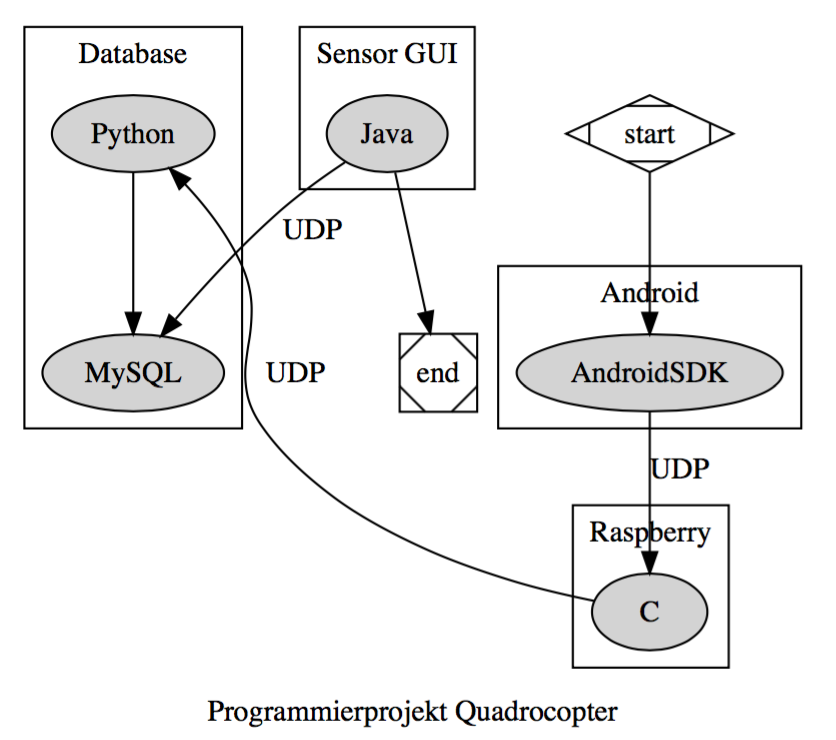
\includegraphics[width=0.5\textwidth]{architektur.png} 
\newline 
\piccaption{Hinweis: Dieses Bild wurde mit DOT GraphViz erstellt, siehe Figure 1.}


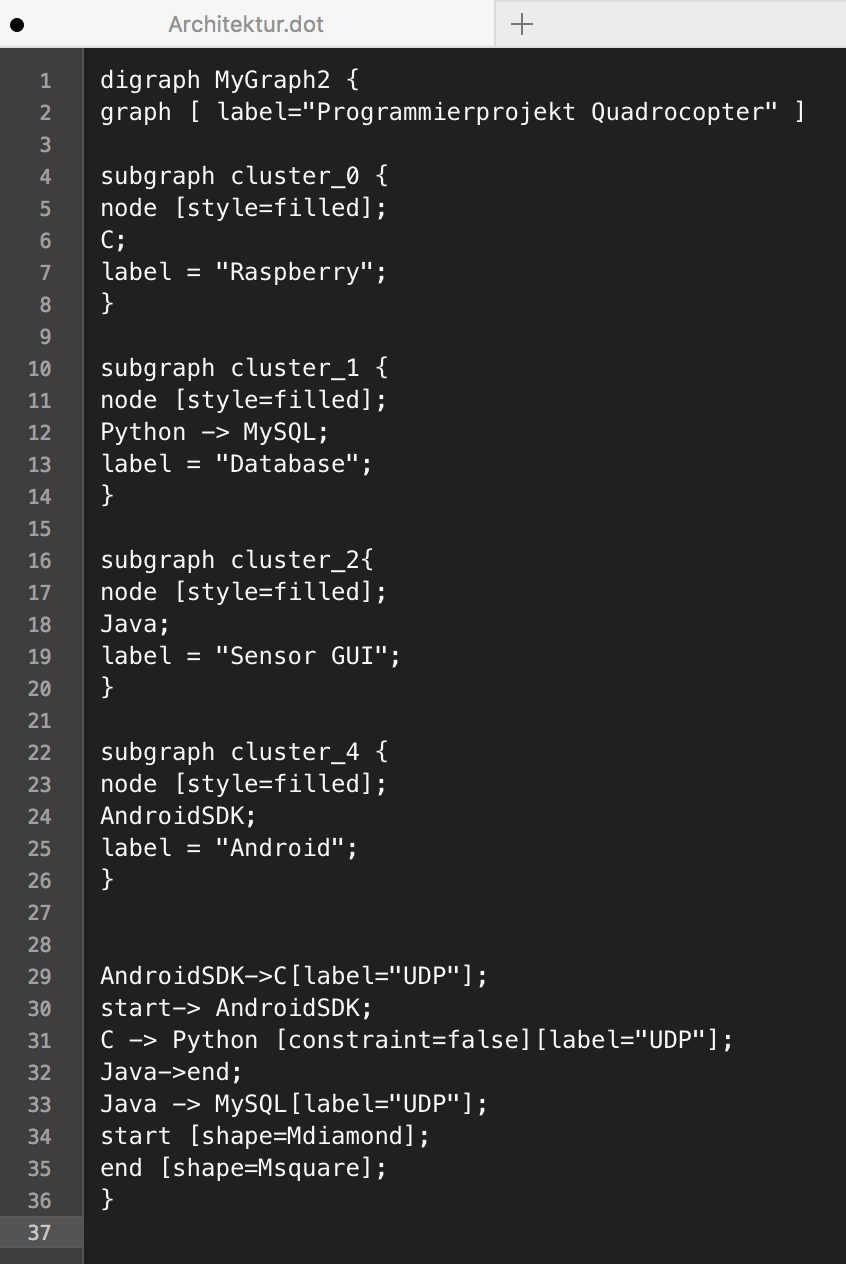
\includegraphics[width=0.4\textwidth]{Architektur_screenshot.png} 
\newline 
\piccaption{Bild: Screenshot Quellcode "Architektur des Projektes"}

%------------------------------------------------

\section{Arbeitsbereich Embedded Systems}

\textbf{Funktionsweise:} \newline 
Das Rasperry Pi bekommt seine Befehl von der App via UDP und führt je nach Protokoll unterschiedliche Funktionen aus.  Jeder der vier Rotoren lässt sich einzeln ansteuern und die Umdrehung festlegen.



Wie das genau aussieht, kann man in Figure 2(Screenshot Motorenansteuerung) sehen.

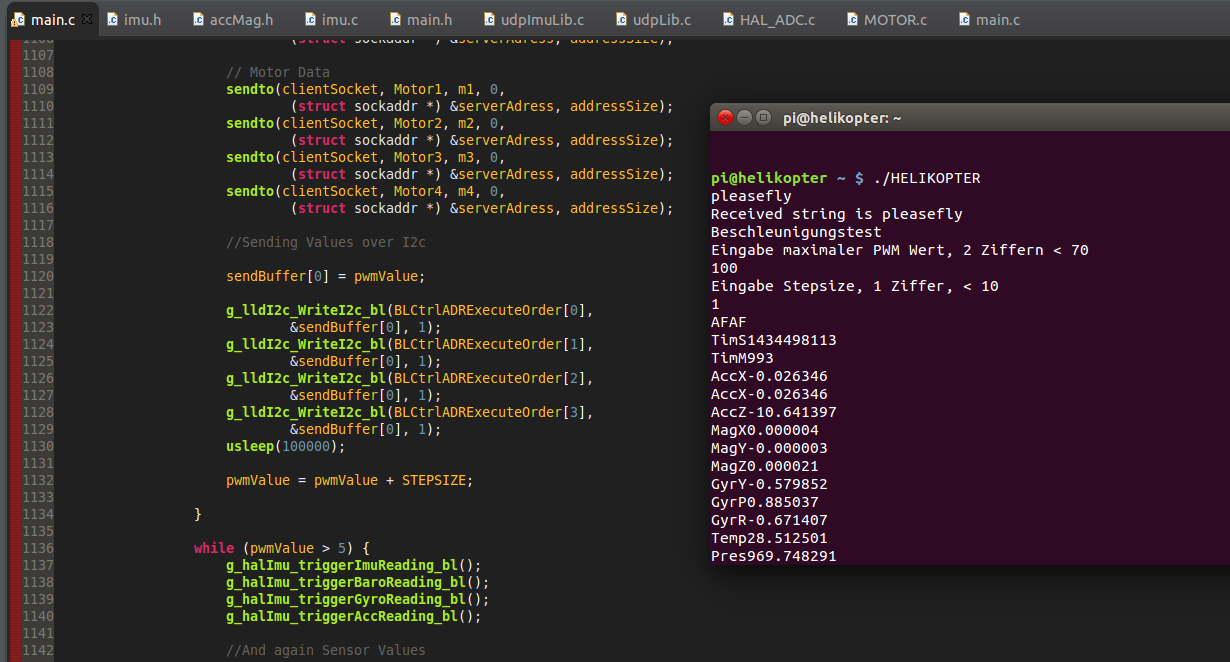
\includegraphics[width=0.45\textwidth]{Raspi.png} 
\newline 
\piccaption{Bild: Screenshot Motorenansteuerung}
}

Zudem möchten wir uns bei Chris Mönch, Oliver Breuning, Jürgen Schmidt für die Rasperry Programmierung bedanken.



\section{Arbeitsbereich Datenbanken}

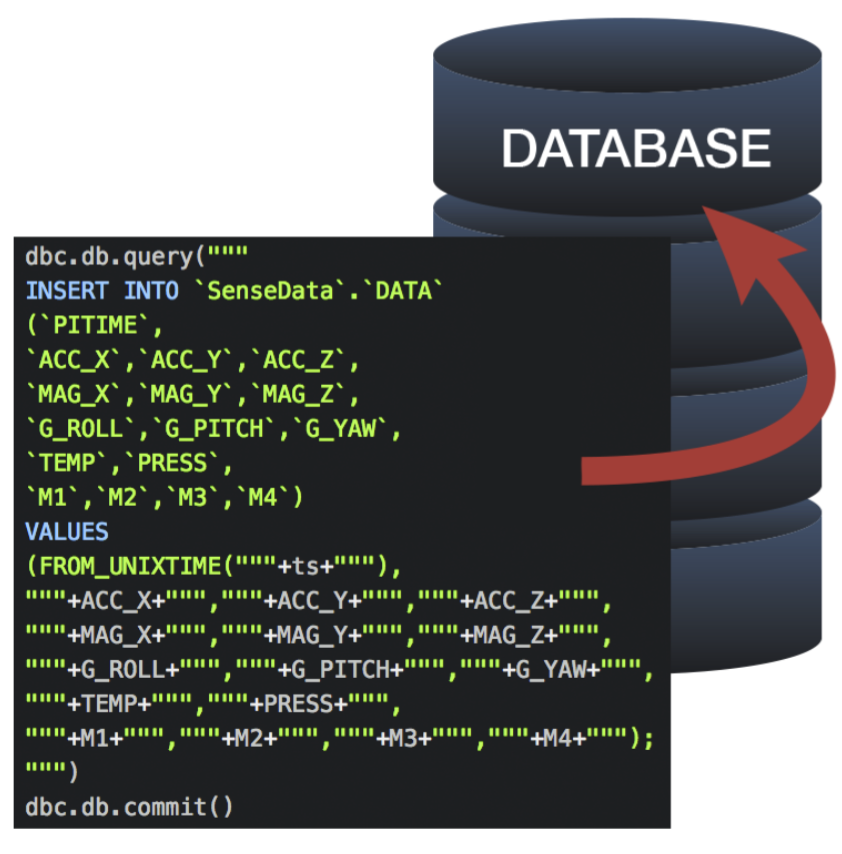
\includegraphics[width=0.5\textwidth]{db-foto.png} 
\newline 
\piccaption{Bild: Screenshot Datenbank}

\section{Arbeitsbereich Graphical User Interface}
\textbf{Funktionsweise:} \newline 
Die GUI liest aus der Datenbank die gespeicherten Sensordaten aus und stellt diese in Graphen dar. Dabei werden aus Konfigurationsdateien die Details für Serverkommunikation, Bezeichnung der Daten und Dimensionen der GUI gelesen. Diese Dateien sind importierbar und können für verschiedene Nutzfälle angepasst werden. Der Nutzer hat die Möglichkeit Daten auszublenden, die dann automatisch auf gute Sichtbarkeit skaliert werden. Außerdem gibt es eine Vielzahl von Optionen durch welche die Anzeige vom Benutzer verbessert werden kann, wie etwa das verschieben, zoomen und pausieren. 
\newline 

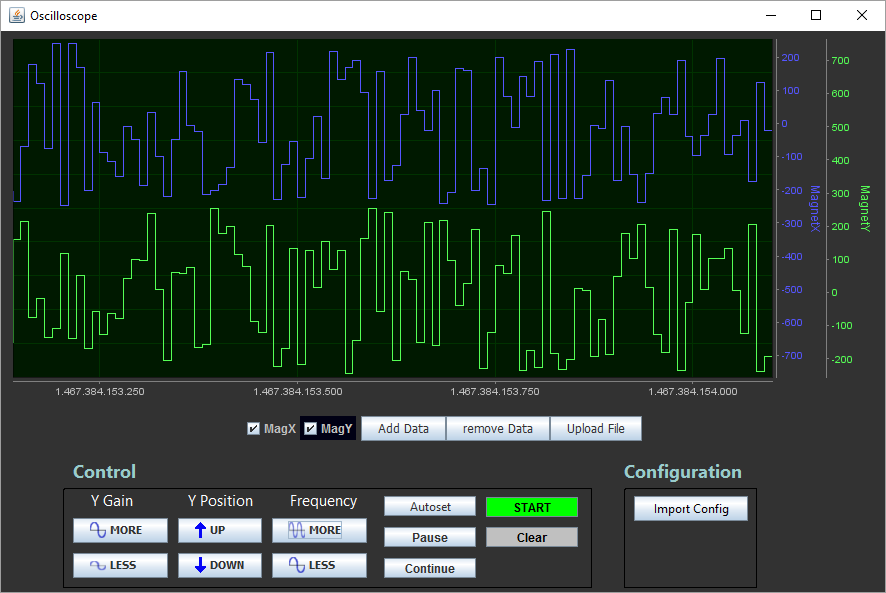
\includegraphics[width=0.5\textwidth]{Oscilloscope.png} 
\piccaption{Bild: Screenshot GUI}

\textbf{Meine Veränderungen/Neuerungen:} \newline 
Meine Aufgabe war es die Daten aus der Datenbank auszulesen und anzuzeigen. Zuerst kam die Implementierung der Konfigurationsdateien, also das erstellen, auslesen und importieren. Danach folgte die automatische Anpassung der Graphen. Diese lagen zuvor übereinander und konnten zu- und weggeschaltet werden. Um eine Überlagerung zu vermeiden, musste die gesamte Skala in die zugehörigen Skalen der aktuell zugeschalteten Graphen unterteilt werden. Schließlich folgte das auslesen der Daten aus der Datenbank. Um eine Echtzeit-Anzeige von Daten zu ermöglichen die auch in Echtzeit in die Datenbank geschrieben werden, muss die Datenbank immer wieder ausgelesen werden um auf neue Daten überprüft zu werden. Da noch keine Dokumentation des Projekts vorhanden war, erstellte ich diese in Javadoc.
\newline 
Neben diesen übergreifenden Aufgaben gab es auch kleine Änderungen, wie etwa Fehlerbehebungen, löschen von nicht mehr benötigten Funktionen, neuordnen von Code und Projektdateien, Änderungen an der GUI und verbessern der Usability.
Für die GUI Programmierung möchte ich mich bei meinen Vorarbeitern Alexander Deitche und Juan-Carlos Barradas-Palmeros bedanken.


\section{Arbeitsbereich Application}
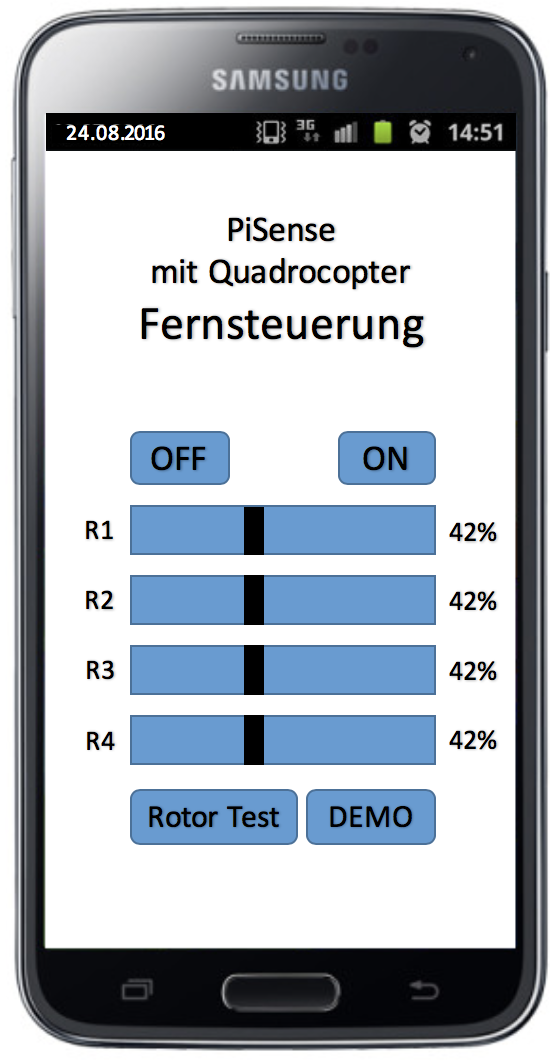
\includegraphics[width=0.4\textwidth]{AppVorlage1.png} 
\newline
\piccaption{Bild: Applikation }

\section{Arbeitsbereich WebProjectManagment}
\textbf{Funktionsweise:} \newline 
Im Bereich WebProjectManagment wurde eine Webapplikation erstellt, in dem es verschiedene Funktionen gibt. Zum einen hat man die Möglichkeit sich zu registrieren und sich danach einzuloggen. Je nachdem welche Berechtigungen man dann hat, hat man Zugriff auf unterschiedliche Inhalte. Zum Beispiel ist das Ticket bearbeiten nur im "admin-modus" möglich.
\newline 
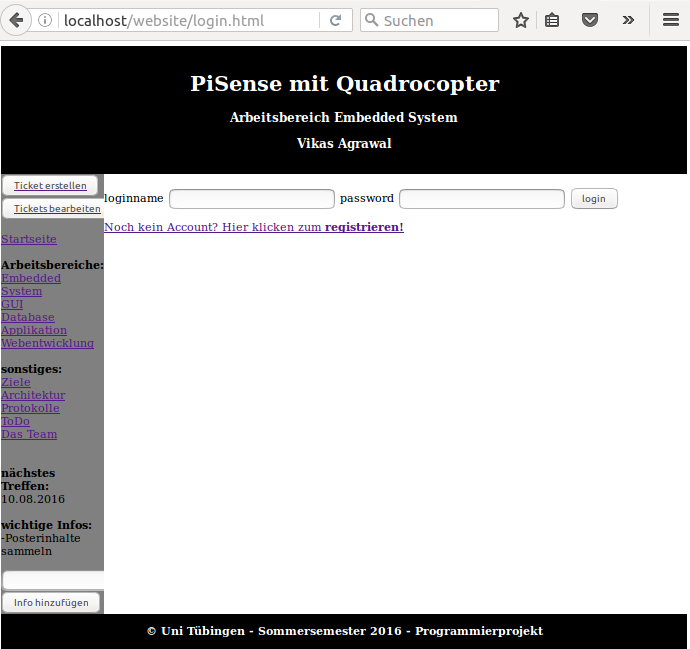
\includegraphics[width=0.5\textwidth]{Bild1.png} 
\piccaption{Bild: Screenshot login.html }
\newline 
\newline 
\textbf{Technische Grundlagen:} \newline 
Die Webapplikation wurde auf einem Apache server gestartet mit Hilfe von LAMP(Linux Apache MySql PHP). Mit LAMP wird auch die Datenbank verwaltet. Die Weboberfläche wurde mit HTML 5 und CSS gestaltet. Die Kommunikation mit MySQL läuft über die Spriktsprache PHP. Um die Übersichtlichkeit der einzelnen Seiten zu optimieren haben wir alle Seiten in PHP geschrieben und am Anfang, sowie am Ende der jeweiligen Seiten ein include("header.php") und include("footer.php") eingefügt, was uns erlaubt die ganze Navigationszeile, das Ticketsystem, den Loginbereich sowie das Grunddesign auszulagern. Der Vorteil liegt darin dass man nur noch eine bzw. zwei Dateien ändern muss und nicht für eine kleine Änderung, alle Seiten welche die Bereiche benutzen. Im Prinzip der gleiche Vorteil welchen wir auch durch die CSS auslagerung haben. Möchten wir unser design ändern, können wir dies in der CSS datei machen und alle Seiten, welche ja die style.css eingefügt haben, führen dann die Änderung automatisch aus. 
\newline 
\newline 
\textbf{Die Loginfunktion:} \newline 
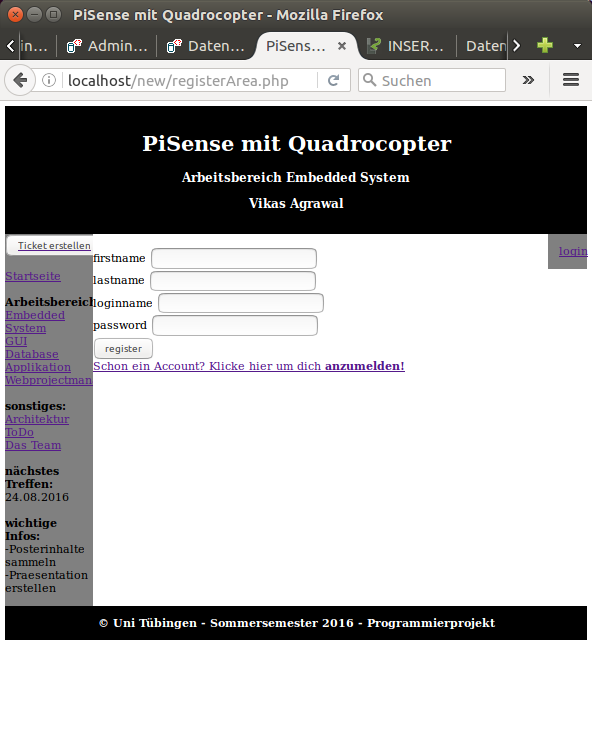
\includegraphics[width=0.5\textwidth]{1.png} 
\piccaption{Bild: Loginbereich }
\newline 
\newline 
\newline 
Die Loginfunktion funktioniert wie folgt: Die Anmeldedaten werden über die GET methode in der Datei loginArea.php an die login.php geschickt und dort mit Daten aus der Datenbank verglichen. Wenn der loginname und das Passwort übereinstimmen, dann wird eine session gestartet und eine Sessionvariable gesetzt, welche speichert ob man angemeldet ist. Wenn alles erfolgreich war, dann wird man auf die index.php seite weitergeleitet via header("Location: index.php"). Dort sieht man nun auf der oberen rechten Seite statt dem login button einen logout button. Falls der login erfolglos war, wird man wieder zu loginArea.php Seite weitergeleitet und der login Button auf der oberen rechten Seite ist bei login.
\newline 
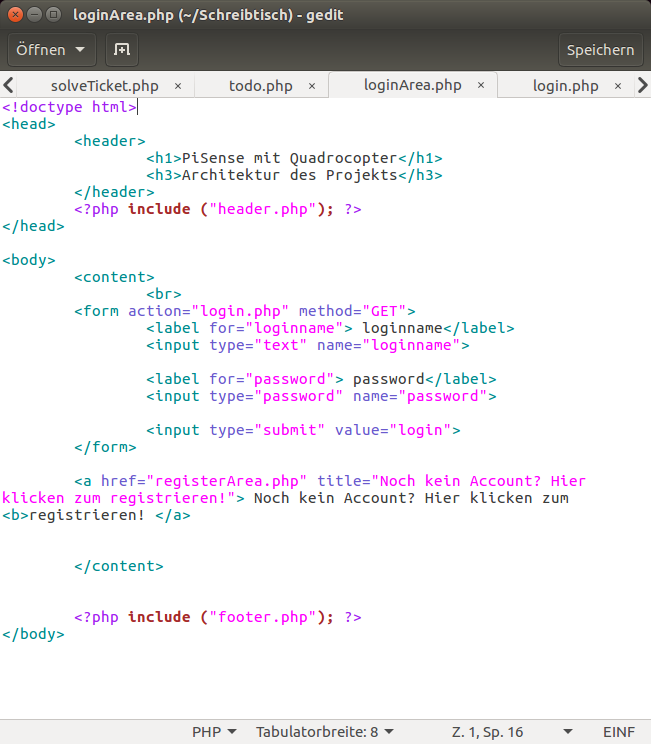
\includegraphics[width=0.5\textwidth]{2.png} 
\piccaption{Bild: Quellcode loginArea.php }
\newline 
\newline 
\newline 
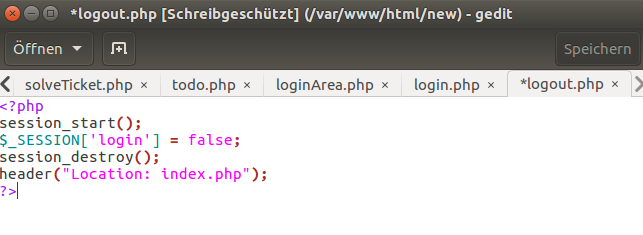
\includegraphics[width=0.5\textwidth]{4.png} 
\piccaption{Bild: Quellcode logout.php }
\newline 
\newline 
\textbf{Das Ticketsystem:} \newline 
Das Ticketsystem wurde entwickelt damit Teammitglieder im Projekt ein Ticket erstellen können und so ihre Fragen und Probleme in der Gruppe stellen. Teammitglieder welche ein bisschen Zeit übrig haben oder sich Zeit schaffen, haben dann die Möglichkeit das Ticket zu bearbeiten.

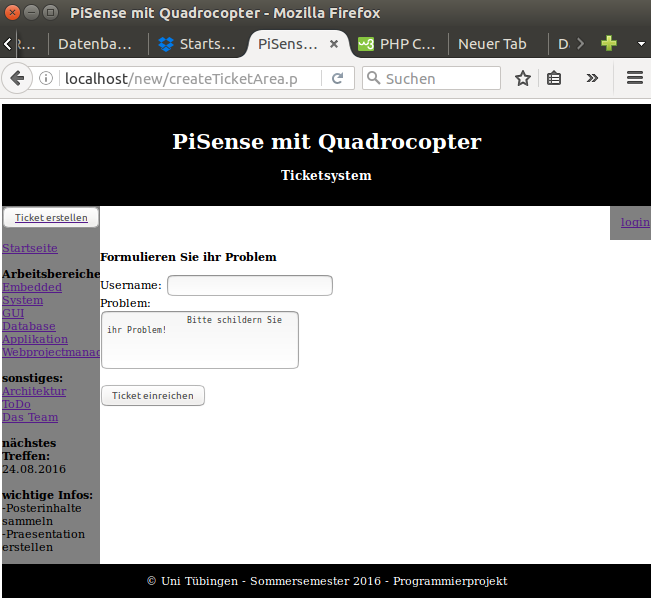
\includegraphics[width=0.5\textwidth]{5.png} 
\piccaption{Bild: Quellcode createTicketArea.php }

%------------------------------------------------
\phantomsection
\section*{zukünftige Ziele:} % The \section*{} command stops section numbering

Real Time Code Generation mit MatLab Simulation




%----------------------------------------------------------------------------------------
%	REFERENCE LIST
%----------------------------------------------------------------------------------------
\phantomsection
\bibliographystyle{unsrt}
\bibliography{sample}

%----------------------------------------------------------------------------------------

\end{document}